\section{A finite lattice carrying all the tests}
\label{lat:section}
\label{sec:lattices}

We now construct the lattice to which Theorem~\ref{cls:chain-rigidity}
will be applied.  All choices in this section precede the choice of a
representing group.  In particular, the length of a test chain will be
chosen using the absolute bound in that Theorem.

Throughout this section, an \emph{original} vertex means a vertex of one
of the two small lattices specified below, before any insertion.  An
original atom of a Boolean lattice need not remain an atom after
insertions; its original meets and joins will, however, be preserved.

\subsection{Two original components and their requested tests}

There are two original components, each with endpoints $0,1$.
For each of the requested pairs below, we shall insert a chain and the
tests from Definition~\ref{cls:tested-chain}.  A forward pair is read
in the displayed order, with bottom $0$; a reverse pair is read in
the dual order, with bottom $1$.

The \emph{Boolean component} is the Boolean lattice $B_4$ of subsets
of a fixed four-element set.  Its forward requested pairs are
\begin{equation}
\label{lat:boolean-forward}
   (v,1)\qquad(0<v<1\text{ original}).
\end{equation}
Its reverse requested pairs are all
\begin{equation}
\label{lat:boolean-reverse}
   (u,v)\qquad(0<v<u<1\text{ original}),
\end{equation}
where a reverse pair is read in the reverse order: its test starts at
$u$ and ends at $v$.  Thus every reverse test is contained in a
forward interval with two proper original endpoints.

The \emph{detector component} has a distinguished original vertex
$X$.  We choose its lower half so that every coatom below $X$ contains
one of two designated vertices $d_1,d_2$.  It is the horizontal sum of
the two chains
\begin{equation}
\label{lat:detector-lower}
   0<p_i<d_i<q_i<X\qquad(i=1,2),
\end{equation}
and its upper half is the horizontal sum of the two chains
\begin{equation}
\label{lat:detector-upper}
   X<e_i<z_i<f_i<1\qquad(i=1,2).
\end{equation}
The two halves are joined at $X$, and we put $z=z_1$.
Its forward requested pairs are
\begin{equation}
\label{lat:detector-forward}
   (d_1,1),\quad(d_2,1),\quad(X,1),
\end{equation}
and its only reverse requested pair is $(z,X)$.
Both $[0,X]$ and $[X,1]$ are already fenced, with two separate
components containing comparable pairs.

\subsection{The lattice properties required in the reduction}

The forward requests will equate the indicated simple labels to the
global top label.  The reverse requests will equate labels inside
reversed upper filters.  These local representations are the ones
that will arise in Section~\ref{ext:section}; a representation of the
entire dual lattice is not needed.  The construction will prove the
following statement while preserving the original Boolean operations.

\begin{proposition}[The decorated lattice]
\label{lat:decorated-lattice}
There is a finite nonempty lattice $L$ with the following properties.
The properties hold in either orientation of $L$, using the
corresponding Boolean and detector components.
\begin{enumerate}[label=\textnormal{(\roman*)}]
\item The lattice contains a bounded copy of the original $B_4$.
  Every proper nonzero original Boolean vertex $v$ has both $[0,v]$
  and $[v,1]$ fenced.  The global interval $[0,1]$ is fenced.
\item There are original detector vertices $d_1,d_2,X,z$ with
  $0<d_i<X<z<1$.  The intervals $[0,d_i]$, $[0,X]$, $[X,1]$ and
  $[z,1]$ are fenced.  Every coatom of $[0,X]$ is above a $d_i$.
\item In any finite subgroup-interval representation $L\cong[D,G]$,
  the simple labels of every proper nonzero original Boolean vertex,
  of $d_1,d_2$, and of $X$ equal the simple label of $G$.
\item Let $0<v<u<1$ be comparable original Boolean vertices.  In any
  finite subgroup-interval representation
  \[
        [v,1]^{\mathrm{op}}\cong[A,U_v],
  \]
  the labels of the vertices corresponding to $u$ and $v$, taken
  relative to the common bottom $A$, are defined and equal.
  The same assertion holds for the detector pair $(z,X)$ in any
  representation $[X,1]^{\mathrm{op}}\cong[A,U_X]$.
\end{enumerate}
In (iv), no representation of the entire dual lattice is assumed.
If several such upper filters have compatible realizations with a
common bottom $A$, the conclusions hold in that compatible system.
\end{proposition}

The remainder of this section constructs this lattice.  We first show
how to add the chain tests while protecting their covering relations,
then combine the forward and reverse tests and choose their length.

\subsection{Private insertions and their persistence properties}

Let $a<b$ in a finite lattice $P$, and let $Q$ be a finite bounded
lattice whose bottom and top are identified with $a$ and $b$.
A \emph{private insertion of $Q$ into $[a,b]$} retains the old orders
and introduces no comparisons between an old vertex and a fresh
interior vertex except those forced through $a$ and $b$.

\begin{lemma}[Private insertion]
\label{lat:insertion}
A private insertion gives a finite lattice and preserves all old meets
and joins.  If $w$ is a fresh interior vertex and $v$ is an old vertex,
then
\begin{equation}
\label{lat:cross-order}
 v\leq w\quad\Longleftrightarrow\quad v\leq a,
 \qquad
 w\leq v\quad\Longleftrightarrow\quad b\leq v.
\end{equation}
An old cover $c\prec d$ is destroyed by the insertion if and only if
the insertion has endpoints $a=c$, $b=d$ and has a nonempty interior.
\end{lemma}

\begin{proof}
The prescribed order is transitive: every route from an old vertex into
the fresh interior passes through $a$, and every route back passes
through $b$.  This proves \eqref{lat:cross-order} and antisymmetry.
For an old vertex $v$ incomparable with a fresh interior vertex $w$,
the cross operations are
\[
 v\wedge w=v\wedge a,
 \qquad v\vee w=v\vee b,
\]
where the operations on the right are those of $P$.  In the comparable
cases, the smaller and larger vertices give the meet and join.
For two fresh vertices, the operations in $Q$ remain their operations:
an old common lower bound lies below $a$, and an old common upper bound
lies above $b$.  An analogous argument shows that an old meet or join
cannot be changed by a new bound.  This proves the lattice assertion.

If a fresh vertex $w$ lies strictly between the old cover $c\prec d$,
then \eqref{lat:cross-order} gives $c\leq a<b\leq d$.
The cover condition forces $a=c$ and $b=d$.  Conversely, an insertion
with those endpoints and a fresh interior vertex destroys the cover.
\end{proof}

A \emph{chain insertion with $k$ interior vertices} means a private
insertion of a chain with exactly $k$ fresh interior vertices.  A
\emph{fencing insertion} means two separate chain insertions, each
with exactly two fresh interior vertices, into the same interval.
In particular, these are nontrivial fences in the sense used in
Lemma~\ref{frm:normal-test}.

\begin{lemma}[Persistent fences]
\label{lat:persistent-fence}
Suppose the proper part of an interval $[a,b]$ has two different
components in its comparability graph, each containing two strictly
comparable vertices.  Then $[a,b]$ is fenced.  This property persists
under any finite sequence of private insertions into the surrounding
lattice.  In particular, a fencing insertion makes an interval fenced
permanently.
\end{lemma}

\begin{proof}
Vertices in different components of the proper comparability graph
have meet $a$ and join $b$.  Indeed, a common lower bound strictly above
$a$, or a common upper bound strictly below $b$, would connect them.
For a given interior vertex, choose the two comparable vertices in one
of the two specified components different from its own.  They are its
required complements.

Consider an insertion into $[c,d]$.  A fresh vertex can belong to
$[a,b]$ only if $a\leq c<d\leq b$, by
Lemma~\ref{lat:insertion}.  If both $c,d$ are proper vertices of
$[a,b]$, they lie in the same comparability component.  All comparisons
from the new interior to the old proper part then enter that component.
The same is true if just one of $c,d$ is proper.  If $c=a$ and $d=b$,
the new interior has no comparisons with the old proper part.
Thus no insertion merges two old components.  The two reserved
comparable pairs survive, proving persistence.  A fencing insertion
supplies two such separate components.
\end{proof}

We shall make several insertions in a \emph{batch}.  This means a
finite list of private insertions all of whose endpoints were present
before the batch.  Perform them in any fixed order.  All their fresh
vertices are distinct, and Lemma~\ref{lat:insertion} applies at every
step.  This convention makes each batch a completely specified finite
operation; it does not call for repeating the batch on its new vertices.

\subsection{The shape of one chain test}

Fix an integer $N\geq2$ and two existing vertices $a<b$.  The following
five batches constitute the \emph{shape construction} for a test on
$(a,b)$.  All sets of vertices appearing in a later batch are the named
sets from the earlier batches, not all vertices then present.

\begin{enumerate}[label=\textnormal{(\arabic*)}]
\item Insert a chain with $N-1$ fresh interior vertices and name its
  vertices
  \[
    a=x_0<x_1<\cdots<x_N=b.
  \]
\item For each $0\leq i<j\leq N$, insert one fresh vertex $v_{ij}$
  privately into $[x_i,x_j]$.  The designated shortcut is
  $x_i\prec v_{ij}\prec x_j$.
\item Make fencing insertions into every interval in the following
  finite set:
  \[
    \bigl\{[x_i,x_j]:0\leq i<j\leq N\bigr\}
    \ \cup\
    \bigl\{[a,v_{ij}]:1\leq i<j\leq N\bigr\}.
  \]
\item Define the set of upper targets
  \begin{equation}
  \label{lat:targets}
    \mathcal U=
      \{x_j:1\leq j\leq N\}
      \cup\{v_{ij}:1\leq i<j\leq N\}.
  \end{equation}
  For every $u\in\mathcal U$, insert privately into $[a,u]$ the
  bounded lattice with fresh vertices $m_u,t_{u,1},\ldots,t_{u,16}$
  and relations
  \[
    a<m_u<t_{u,k}<u\quad(1\leq k\leq16),
  \]
  with the $t_{u,k}$ pairwise incomparable.  Thus $a<m_u$ and
  $[m_u,u]$ is exactly $M_{16}$ at this stage.
\item For every pair $(a,u)$ with $u\in\mathcal U$, make two separate
  chain insertions with one interior vertex.  Also do so for every
  pair $(c,b)$ with
  \begin{equation}
  \label{lat:saturated-principals}
    c\in\mathcal C=
      \{x_i:0\leq i<N\}
      \cup\{v_{ij}:0\leq i<j<N\}.
  \end{equation}
  Repeated pairs may be listed just once.  The two new vertices for
  a pair $(c,d)$ are its reserved coatom witnesses: they are coatoms
  below $d$, and their meet is $c$.
\end{enumerate}

The vertices $x_i$ and $v_{ij}$ are called the \emph{principal vertices}
of the test.  The vertices $m_u,t_{u,k}$ and the reserved coatom
witnesses are not principal vertices and are not used as endpoints of
any subsequent shape insertion for this test.

\begin{lemma}[A finite shape construction]
\label{lat:shape}
The five batches are finite and have the following properties.
\begin{enumerate}[label=\textnormal{(\roman*)}]
\item Every designated shortcut has both edges as covers.
\item Every $[x_i,x_j]$ is fenced.  For every $u\in\mathcal U$,
      $[a,u]$ is fenced, $a$ is a meet of coatoms below $u$, and
      $a<m_u$ with $[m_u,u]\cong M_{16}$.
\item Every vertex in $\mathcal C$ is a meet of coatoms below $b$.
      Each $v_{iN}$ is itself a coatom below $b$.
\end{enumerate}
No interval $[a,v_{0j}]$ is included in the extra target operations.
The construction introduces at most $27N^2$ vertices.
\end{lemma}

\begin{proof}
Each shortcut edge is a cover immediately after its one-vertex
insertion.  By the cover criterion in Lemma~\ref{lat:insertion}, a
later shape insertion could destroy it only by using that exact edge
as its endpoint pair.  The listed pairs never do so.  The only apparent
possibilities would be $[a,v_{0j}]$, which is excluded from
\eqref{lat:targets}, and $[v_{iN},b]$, which is excluded from
\eqref{lat:saturated-principals}.  This proves (i).

All pair fences are present in the third batch and persist by
Lemma~\ref{lat:persistent-fence}.  The chain targets $x_j$ already have
the fence on $[a,x_j]$ from that batch; the other upper targets are
listed there expressly.  Each reserved coatom witness is fresh when
inserted and is not an endpoint of a subsequent shape insertion.
Its edge to the upper endpoint therefore survives.  Its meet with its
companion remains the lower endpoint, by
Lemma~\ref{lat:insertion}.

When an $M_{16}$ branch is inserted, its interval $[m_u,u]$ has no
other vertices: an old vertex above $m_u$ must be above $u$.
A subsequent shape insertion could add a vertex inside this interval
only if both its endpoints lay in $[m_u,u]$.  None of $m_u,t_{u,k}$
is used subsequently as a shape endpoint.  The remaining possible
endpoint is $u$, which cannot by itself form a nondegenerate interval
inside $[m_u,u]$.  Thus this interval remains exactly $M_{16}$.
These arguments give (ii) and (iii).

For completeness, the numbers of new vertices in the first four
batches are respectively
\[
 N-1,\qquad \frac{N(N+1)}2,\qquad 4N^2,
 \qquad \frac{17N(N+1)}2.
\]
The fifth batch adds at most $2N(N+1)$ vertices.  Their sum is
$15N^2+12N-1\leq27N^2$.
\end{proof}

The exclusions involving $v_{0j}$ and $v_{iN}$ are necessary.
Inserting a fence into either of their designated cover edges would
destroy the two-edge shortcut.  The target set
\eqref{lat:targets} is exactly the one required by
Theorem~\ref{cls:chain-rigidity}; no test at a target $v_{0j}$ is
needed there.

\subsection{Combining the forward and reverse tests}

Here is the complete construction for either original component $C$.
First perform the five shape batches for all its forward requested
pairs, using fresh vertices for every pair.  One may perform a batch
for all pairs before passing to the next batch.  Then apply the same
five batches in the dual lattice for all reverse requested pairs,
again with disjoint fresh vertices.  In each case a
private insertion is made in the order currently being used; its dual
is a private insertion in the forward lattice.

Let $C^{\mathrm{sh}}_N$ be the finite lattice now obtained, and freeze
its vertex set.  Define two subsets of this frozen set:
\begin{align}
\label{lat:label-sets}
 \mathcal F_C
   &=\bigcup_{(a,1)\text{ forward requested}}
          [a,1]_{C^{\mathrm{sh}}_N},\\
 \mathcal R_C
   &=\bigcup_{(u,v)\text{ reverse requested}}
          [v,u]_{C^{\mathrm{sh}}_N}.
\end{align}
The following is a \emph{single final batch}, with every endpoint
chosen from this frozen set:
\begin{itemize}
\item make a fencing insertion into $[0,t]$ for every
  $t\in\mathcal F_C\setminus\{1\}$;
\item make a fencing insertion into $[t,1]$ for every
  $t\in\mathcal R_C$.
\end{itemize}
In the detector omit the first insertion when $t=X$, since $[0,X]$
is already fenced.  No insertion into $[0,X]$ is made anywhere in the
construction.  Denote the resulting component by $C_N$.

We emphasize that the new vertices of this final batch are not added
to $\mathcal F_C$ or $\mathcal R_C$.  The next lemma proves that no
such closure operation is needed.

\begin{lemma}[Simultaneous tests and the final batch]
\label{lat:simultaneous}
For either component $C_N$, all the following statements hold.
\begin{enumerate}[label=\textnormal{(\roman*)}]
\item Every forward shape test retains all conclusions of
  Lemma~\ref{lat:shape}.  Its principal vertices other than $1$ have
  fenced intervals from $0$.
\item Every reverse shape test retains all conclusions of
  Lemma~\ref{lat:shape} in the reverse order.  Every vertex in each
  of its comparison intervals has a fenced interval from the reverse
  base $1$.
\item For a forward chosen chain and any $i<j$, every vertex
  $t\in[x_i,x_j]$, except possibly $t=1$, satisfies one of the
  following alternatives:
  \begin{enumerate}[label=\textnormal{(\alph*)}]
  \item $[0,t]$ is fenced;
  \item there is a vertex $s$ with $x_i\leq s<t$, with $[0,s]$
    fenced, such that every vertex of $[0,t]$ is comparable to $s$.
  \end{enumerate}
\item In the detector the coatoms of $[0,X]$ are exactly $q_1,q_2$.
  In particular, each contains one of $d_1,d_2$ below it.  The
  intervals $[0,X]$ and $[X,1]$ remain fenced.
\end{enumerate}
The construction is finite.  If $C$ has $q_0$ vertices and altogether
$h$ requested pairs in the two directions, then
\[
             |C_N|\leq9(q_0+27hN^2).
\]
\end{lemma}

\begin{proof}
We first record how the two shape constructions are separated.  Every
fresh vertex of a forward shape construction lies below no proper
original vertex.  This follows inductively from
\eqref{lat:cross-order}: its upper insertion endpoint is either $1$
or an earlier fresh forward vertex with the same property.  In
contrast, every vertex of a reverse shape construction lies in a
forward interval $[v,u]$ with $0<v<u<1$ original.  Thus every vertex
of $\mathcal R_C$ lies below a proper original upper bound, and no
fresh forward vertex belongs to $\mathcal R_C$.

These observations also show that the shape constructions do not
spoil each other's designated intervals.  Different forward tests
have disjoint fresh interiors; their only shared shape endpoints are
original vertices and $1$.  Hence neither uses a fresh endpoint of
the other's designated cover.  No reverse shape insertion can use
such a forward endpoint as its lower endpoint, since it lies below
a proper original upper bound.  For reverse tests, two different
tests again have disjoint fresh interiors and share only original
endpoints.  Lemma~\ref{lat:insertion} therefore protects their covers.
The same argument protects the exact $M_{16}$ intervals: a shape
insertion could enter one only if its two endpoints lay inside it,
whereas its fresh bottom and atoms are never shape endpoints.
Fences persist by Lemma~\ref{lat:persistent-fence}.

We next check the final batch.  A new vertex of $[0,t]$ belongs to no
comparison interval $[a,b]$ with $a>0$, by
\eqref{lat:cross-order}.  A new vertex of $[t,1]$ can belong to such
a comparison only if $b=1$ and $a\leq t$.  The lower endpoints of
the latter insertions are in $\mathcal R_C$, and consequently lie
below proper original upper bounds.

In particular, a reverse fence cannot subdivide a fresh forward
coatom edge $c\prec1$: that would require its lower endpoint to be
exactly $c$, which lies below no proper original vertex.  A forward
cover with a proper upper endpoint cannot be subdivided by an
insertion ending at $1$.  Thus all forward shortcut edges and all
reserved coatom witnesses survive.  A forward $M_{16}$ interval with
proper upper endpoint cannot be entered by a reverse fence.  If its
upper endpoint is $1$, its fresh bottom lies below no proper original
vertex; hence no point of $\mathcal R_C$ lies above that bottom.
So this $M_{16}$ interval also remains exact.  Forward base insertions
cannot enter any of these positive-bottom intervals.

All reverse comparison intervals have two proper original bounds in
the forward order.  Neither kind of final insertion can add a vertex
to such an interval: an insertion beginning at $0$ cannot do so, and
an insertion ending at $1$ cannot do so.  Their covers, witnesses and
exact $M_{16}$ intervals are therefore unchanged.  The final reverse
fences label every vertex in each reverse comparison interval by
the definition of $\mathcal R_C$.  All required forward principal
vertices belong to $\mathcal F_C$; the sole omitted proper target is
the detector $X$, whose lower interval was fenced at the outset.
This proves (i) and (ii).

For (iii), an old vertex in a forward comparison belongs to
$\mathcal F_C$, so its lower interval is fenced, with the stated
exception for the global top.  The only possible new vertex is an
interior vertex $w$ of a final reverse fencing insertion into $[s,1]$.
If $x_i\leq w$, then $x_i\leq s$ by
\eqref{lat:cross-order}.  Every vertex below $w$ either lies below
$s$ or lies on the same private chain above $s$.  This assertion also
includes vertices of other insertions in the final batch: a point
from another branch can be below $w$ only by passing through the old
endpoint $s$.  Thus $s$ is comparable to every vertex of $[0,w]$.
Moreover $s\in\mathcal F_C$, since $x_i\leq s<1$, and its lower
interval is fenced.  This is exactly alternative (b), including the
requirement that the bottleneck lie above the lower chosen chain
vertex.  It proves closure of the normal-group tests without any new
round of insertions.

For (iv), no shape insertion introduces a point strictly below $X$.
Forward fresh points lie below no proper original vertex, and reverse
shape insertions in the detector are contained in $[X,z]$.
A final insertion ending strictly below $X$ introduces only points
below that endpoint, so it cannot create a new coatom of $[0,X]$.
A final insertion ending above $X$ introduces no new point below $X$.
The only remaining possibility would be an insertion into $[0,X]$,
which was omitted.  Hence the original covers $q_i\prec X$ are
precisely the coatoms of the lower half.  Its two separate original
branches, and those of the upper half, still give fences by
Lemma~\ref{lat:persistent-fence}.

Finally, Lemma~\ref{lat:shape} bounds the size before the final batch
by $q=q_0+27hN^2$.  Each of $\mathcal F_C$ and $\mathcal R_C$ has
at most $q$ members, and each fencing insertion adds four vertices.
The final size is at most $q+4q+4q=9q$.  This also proves finiteness
directly from the displayed batches.
\end{proof}

\subsection{Assembly and proof of the lattice properties}

Let $B_N$ and $E_N$ denote respectively the decorated Boolean and
detector components just constructed.  Define $L_N$ to be the
horizontal sum
\begin{equation}
\label{lat:horizontal-sum}
       L_N=B_N\boxplus B_N^{\mathrm{op}}
                  \boxplus E_N\boxplus E_N^{\mathrm{op}},
\end{equation}
identifying only the common endpoints $0,1$.  Interiors of different
components are incomparable, with cross meet $0$ and cross join $1$.
The order reversal exchanging each component with its opposite is
an order anti-isomorphism of $L_N$.  Thus $L_N$ is self-dual.

Every component has two comparable proper original vertices.  The
global interval $[0,1]$ is therefore fenced: for a vertex in one
component, take a comparable pair in a different component.  A
comparison with a proper starting point, or a principal interval with
a proper upper endpoint, contains no interior vertex from a different
component.  Thus horizontal summation preserves every local property
proved above, and supplies the previously deferred label at the
global top.

\begin{proof}[Proof of Proposition~\ref{lat:decorated-lattice}]
Let $B$ be the absolute chain threshold of
Theorem~\ref{cls:chain-rigidity}, and choose the single integer
$N=\max\{2,\lceil B\rceil\}$.  Construct $L=L_N$ by the finite operations above.
This choice is independent of every possible representing group.
Finiteness follows from Lemma~\ref{lat:simultaneous} and
\eqref{lat:horizontal-sum}; no limiting lattice is used.

All original lattice operations survive by
Lemma~\ref{lat:insertion}.  Every proper original Boolean vertex is
an endpoint of a forward requested pair and of a reverse requested
pair, so its two principal intervals receive the required fences.
The detector statements follow from
Lemma~\ref{lat:simultaneous}.  This gives (i) and (ii).

For (iii), take a finite representation $[D,G]$.  By
Lemma~\ref{frm:labels}, the global fence and the required principal
fences provide all forward labels.  In every forward requested test,
the sequence $x_0<\cdots<x_N$ and its private shortcuts have the
shape required by Theorem~\ref{cls:chain-rigidity}, including its
nonconsecutive shortcuts.  The interval $[x_i,x_j]$ is fenced;
every target in \eqref{lat:targets} has its bottom saturation,
fence, and exact positive-bottom $M_{16}$ interval; and all the
specified principal vertices are meets of coatoms below the largest
endpoint, with $v_{iN}$ themselves coatoms.  Finally,
Lemma~\ref{lat:simultaneous}(iii), together with the global fence,
verifies condition~\ref{cls:test-normal} at every vertex of every comparison:
either its lower interval is fenced or it has the specified labelled
bottleneck above the lower chain vertex.  In the latter case,
Corollary~\ref{frm:bottleneck} supplies the required soluble-normal
and commuting-normal consequences.  All hypotheses of the
chain Theorem hold, and $N\geq B$ forces equality of its endpoint
types.  The forward requested pairs are precisely
\eqref{lat:boolean-forward} and \eqref{lat:detector-forward}, giving
the asserted equalities.

For (iv), fix one of the indicated actual upper-filter
representations.  Its least lattice vertex is the former $1$, and
its group bottom is $A$.  The entire reverse test for $(u,v)$ lies
inside this upper filter.  Its principal labels come from intervals
$[w,1]^{\mathrm{op}}$, which are fenced by the final reverse batch.
All vertices of its comparison intervals have those fences, by
Lemma~\ref{lat:simultaneous}(ii).  The reverse shape construction
supplies all the other hypotheses of the same chain Theorem.
Consequently the two endpoint labels, now taken relative to $A$,
are equal.  The proof for $(z,X)$ is identical.  If the actual
intervals are compatible, their common subgroups and their labels
are the same on overlaps; the argument makes no additional choice of
a representation and thus applies simultaneously.

Finally, the order reversal exchanging the paired components in
\eqref{lat:horizontal-sum} supplies the same Boolean and detector
data in the other orientation.  This proves the last assertion.
\end{proof}

We record explicitly the Boolean incidence used in the final gluing
argument; Figure~\ref{fig:boolean-faces} shows its proper faces.  In the reverse original $B_4$, fix an original atom $x$ and
let $a_1,\ldots,a_3$ be the other original atoms.  Put
\[
                    u_i=x\vee a_i\qquad(1\leq i\leq3),
\]
with operations in that reverse Boolean copy.  Each $u_i\vee u_j$
for $i\ne j$ has rank three and is proper, while
$\bigvee_{i=1}^3u_i$ is the reverse top.  Every proper original
Boolean vertex is the join of the original atoms below it.  These
equalities are still equalities in the full decorated lattice, since
all insertions preserve old operations.  Thus the local proper joins
and the incompatible total join required later are present in the
single finite lattice of Proposition~\ref{lat:decorated-lattice}.

\begin{figure}[htbp]
\centering
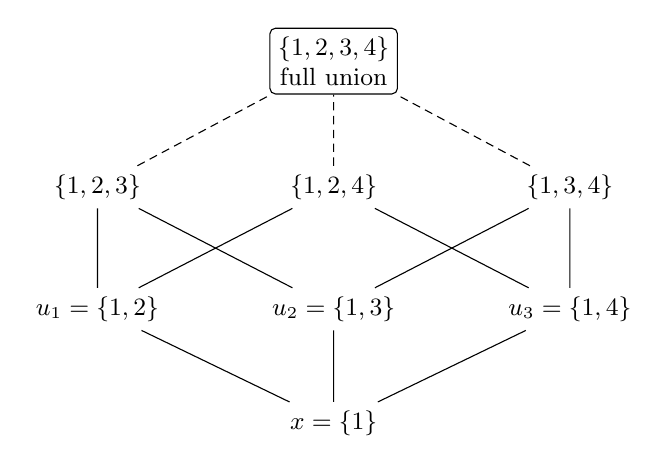
\begin{tikzpicture}[x=1cm,y=1cm,
  face/.style={fill=white,inner sep=3pt},
  every node/.style={font=\small}]
\node[face] (x) at (0,0) {$x=\{1\}$};
\node[face] (u1) at (-3,1.45) {$u_1=\{1,2\}$};
\node[face] (u2) at (0,1.45) {$u_2=\{1,3\}$};
\node[face] (u3) at (3,1.45) {$u_3=\{1,4\}$};
\node[face] (w12) at (-3,3) {$\{1,2,3\}$};
\node[face] (w13) at (0,3) {$\{1,2,4\}$};
\node[face] (w23) at (3,3) {$\{1,3,4\}$};
\node[face,draw,rounded corners=2pt,align=center] (all) at (0,4.6)
  {$\{1,2,3,4\}$\\full union};
\draw (x)--(u1) (x)--(u2) (x)--(u3);
\draw (u1)--(w12) (u1)--(w13);
\draw (u2)--(w12) (u2)--(w23);
\draw (u3)--(w13) (u3)--(w23);
\draw[densely dashed] (w12)--(all) (w13)--(all) (w23)--(all);
\end{tikzpicture}
\caption{The original Boolean faces containing $x$. Each pair among
$u_1,u_2,u_3$ has a proper union, but their total union is full.
All displayed subset relations survive the private insertions.
In the extension configuration of Proposition~\ref{ext:reduction},
solid edges correspond to restrictions of compatible homomorphisms
on actual nested domains. The dashed edges reach the full union,
for which a common extension is forbidden.}
\label{fig:boolean-faces}
\end{figure}

